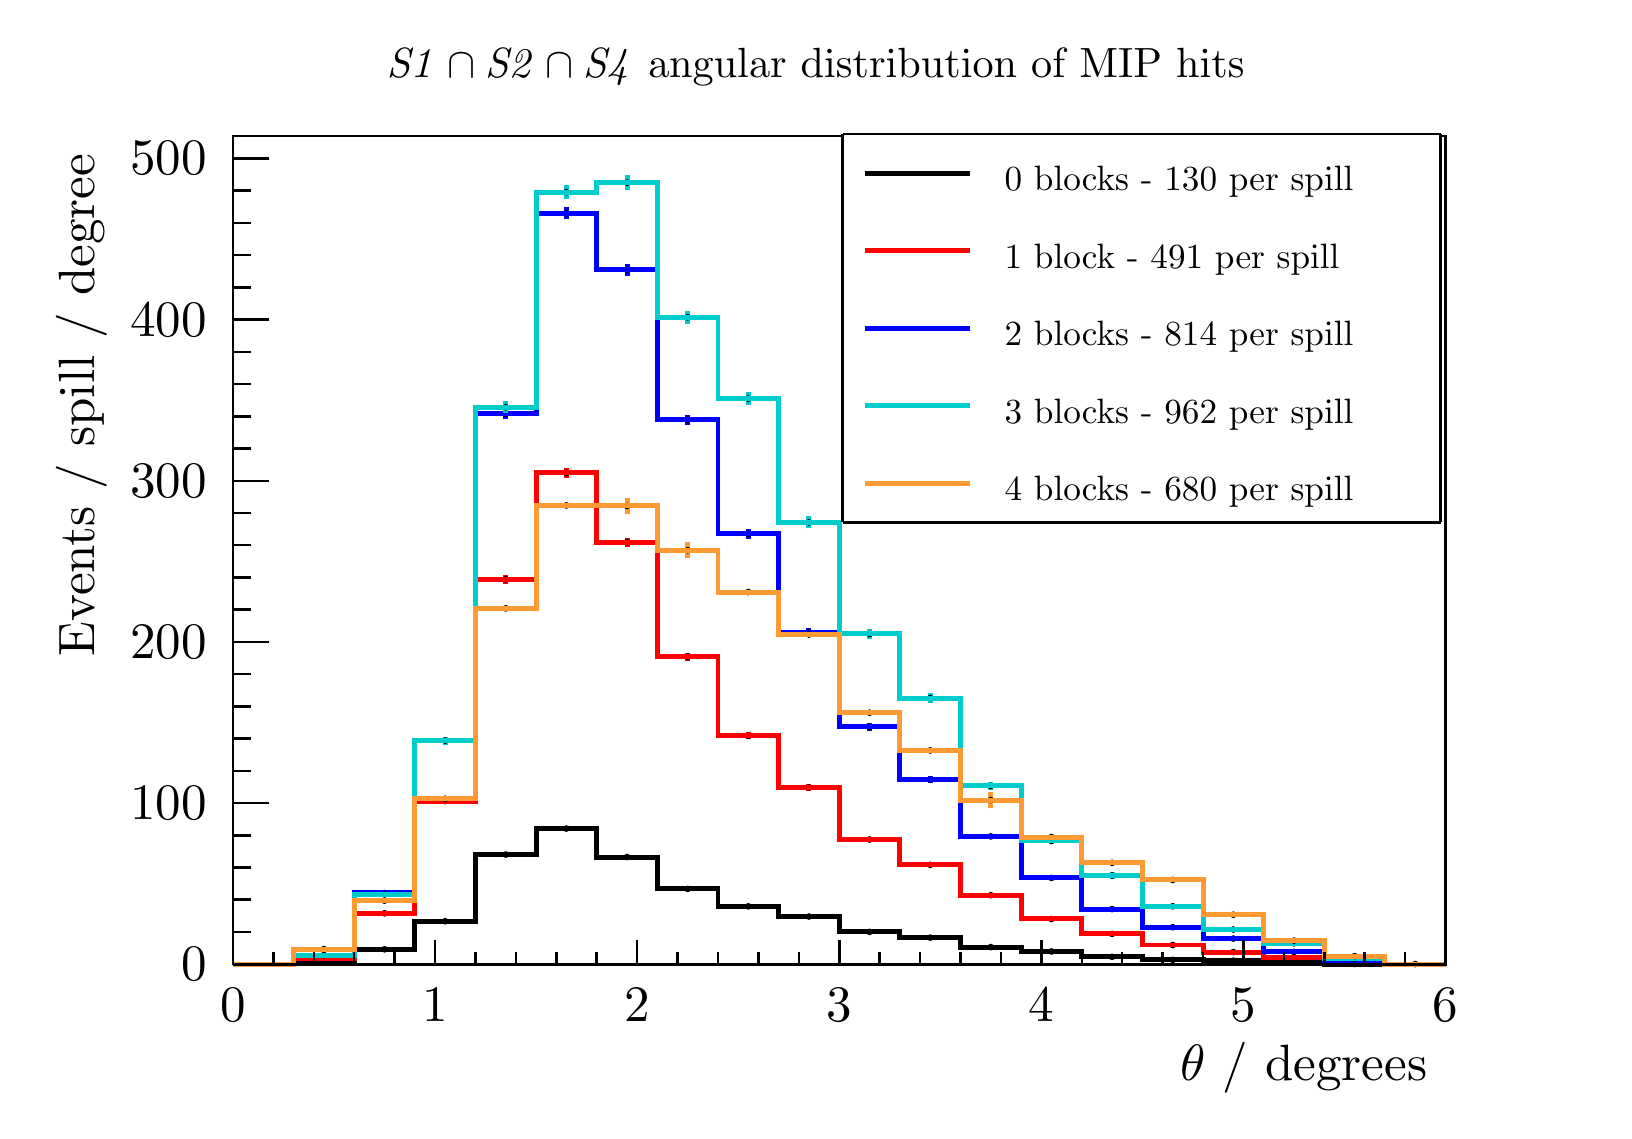
\begin{tikzpicture}
\pgfdeclareplotmark{cross} {
\pgfpathmoveto{\pgfpoint{-0.3\pgfplotmarksize}{\pgfplotmarksize}}
\pgfpathlineto{\pgfpoint{+0.3\pgfplotmarksize}{\pgfplotmarksize}}
\pgfpathlineto{\pgfpoint{+0.3\pgfplotmarksize}{0.3\pgfplotmarksize}}
\pgfpathlineto{\pgfpoint{+1\pgfplotmarksize}{0.3\pgfplotmarksize}}
\pgfpathlineto{\pgfpoint{+1\pgfplotmarksize}{-0.3\pgfplotmarksize}}
\pgfpathlineto{\pgfpoint{+0.3\pgfplotmarksize}{-0.3\pgfplotmarksize}}
\pgfpathlineto{\pgfpoint{+0.3\pgfplotmarksize}{-1.\pgfplotmarksize}}
\pgfpathlineto{\pgfpoint{-0.3\pgfplotmarksize}{-1.\pgfplotmarksize}}
\pgfpathlineto{\pgfpoint{-0.3\pgfplotmarksize}{-0.3\pgfplotmarksize}}
\pgfpathlineto{\pgfpoint{-1.\pgfplotmarksize}{-0.3\pgfplotmarksize}}
\pgfpathlineto{\pgfpoint{-1.\pgfplotmarksize}{0.3\pgfplotmarksize}}
\pgfpathlineto{\pgfpoint{-0.3\pgfplotmarksize}{0.3\pgfplotmarksize}}
\pgfpathclose
\pgfusepathqstroke
}
\pgfdeclareplotmark{cross*} {
\pgfpathmoveto{\pgfpoint{-0.3\pgfplotmarksize}{\pgfplotmarksize}}
\pgfpathlineto{\pgfpoint{+0.3\pgfplotmarksize}{\pgfplotmarksize}}
\pgfpathlineto{\pgfpoint{+0.3\pgfplotmarksize}{0.3\pgfplotmarksize}}
\pgfpathlineto{\pgfpoint{+1\pgfplotmarksize}{0.3\pgfplotmarksize}}
\pgfpathlineto{\pgfpoint{+1\pgfplotmarksize}{-0.3\pgfplotmarksize}}
\pgfpathlineto{\pgfpoint{+0.3\pgfplotmarksize}{-0.3\pgfplotmarksize}}
\pgfpathlineto{\pgfpoint{+0.3\pgfplotmarksize}{-1.\pgfplotmarksize}}
\pgfpathlineto{\pgfpoint{-0.3\pgfplotmarksize}{-1.\pgfplotmarksize}}
\pgfpathlineto{\pgfpoint{-0.3\pgfplotmarksize}{-0.3\pgfplotmarksize}}
\pgfpathlineto{\pgfpoint{-1.\pgfplotmarksize}{-0.3\pgfplotmarksize}}
\pgfpathlineto{\pgfpoint{-1.\pgfplotmarksize}{0.3\pgfplotmarksize}}
\pgfpathlineto{\pgfpoint{-0.3\pgfplotmarksize}{0.3\pgfplotmarksize}}
\pgfpathclose
\pgfusepathqfillstroke
}
\pgfdeclareplotmark{newstar} {
\pgfpathmoveto{\pgfqpoint{0pt}{\pgfplotmarksize}}
\pgfpathlineto{\pgfqpointpolar{44}{0.5\pgfplotmarksize}}
\pgfpathlineto{\pgfqpointpolar{18}{\pgfplotmarksize}}
\pgfpathlineto{\pgfqpointpolar{-20}{0.5\pgfplotmarksize}}
\pgfpathlineto{\pgfqpointpolar{-54}{\pgfplotmarksize}}
\pgfpathlineto{\pgfqpointpolar{-90}{0.5\pgfplotmarksize}}
\pgfpathlineto{\pgfqpointpolar{234}{\pgfplotmarksize}}
\pgfpathlineto{\pgfqpointpolar{198}{0.5\pgfplotmarksize}}
\pgfpathlineto{\pgfqpointpolar{162}{\pgfplotmarksize}}
\pgfpathlineto{\pgfqpointpolar{134}{0.5\pgfplotmarksize}}
\pgfpathclose
\pgfusepathqstroke
}
\pgfdeclareplotmark{newstar*} {
\pgfpathmoveto{\pgfqpoint{0pt}{\pgfplotmarksize}}
\pgfpathlineto{\pgfqpointpolar{44}{0.5\pgfplotmarksize}}
\pgfpathlineto{\pgfqpointpolar{18}{\pgfplotmarksize}}
\pgfpathlineto{\pgfqpointpolar{-20}{0.5\pgfplotmarksize}}
\pgfpathlineto{\pgfqpointpolar{-54}{\pgfplotmarksize}}
\pgfpathlineto{\pgfqpointpolar{-90}{0.5\pgfplotmarksize}}
\pgfpathlineto{\pgfqpointpolar{234}{\pgfplotmarksize}}
\pgfpathlineto{\pgfqpointpolar{198}{0.5\pgfplotmarksize}}
\pgfpathlineto{\pgfqpointpolar{162}{\pgfplotmarksize}}
\pgfpathlineto{\pgfqpointpolar{134}{0.5\pgfplotmarksize}}
\pgfpathclose
\pgfusepathqfillstroke
}
\definecolor{c}{rgb}{1,1,1};
\draw [color=c, fill=c] (0,0) rectangle (20,13.6676);
\draw [color=c, fill=c] (2.6,1.77679) rectangle (18,12.3009);
\definecolor{c}{rgb}{0,0,0};
\draw [c,line width=0.9] (2.6,1.77679) -- (2.6,12.3009) -- (18,12.3009) -- (18,1.77679) -- (2.6,1.77679);
\definecolor{c}{rgb}{1,1,1};
\draw [color=c, fill=c] (2.6,1.77679) rectangle (18,12.3009);
\definecolor{c}{rgb}{0,0,0};
\draw [c,line width=0.9] (2.6,1.77679) -- (2.6,12.3009) -- (18,12.3009) -- (18,1.77679) -- (2.6,1.77679);
\definecolor{c}{rgb}{0,0,0.6};
\draw [c,line width=0.9] (2.6,1.78082) -- (3.37,1.78082) -- (3.37,1.78082) -- (4.14,1.78082) -- (4.14,1.78082) -- (4.91,1.78082) -- (4.91,1.78082) -- (5.68,1.78082) -- (5.68,1.78082) -- (6.45,1.78082) -- (6.45,1.78082) -- (7.22,1.78082) --
 (7.22,1.78082) -- (7.99,1.78082) -- (7.99,1.78082) -- (8.76,1.78082) -- (8.76,1.78082) -- (9.53,1.78082) -- (9.53,1.78082) -- (10.3,1.78082) -- (10.3,1.78082) -- (11.07,1.78082) -- (11.07,1.78082) -- (11.84,1.78082) -- (11.84,1.78082) --
 (12.61,1.78082) -- (12.61,1.78082) -- (13.38,1.78082) -- (13.38,1.78082) -- (14.15,1.78082) -- (14.15,1.78082) -- (14.92,1.78082) -- (14.92,1.78082) -- (15.69,1.78082) -- (15.69,1.78082) -- (16.46,1.78082) -- (16.46,1.78082) -- (17.23,1.78082) --
 (17.23,1.78082) -- (18,1.78082);
\definecolor{c}{rgb}{0,0,0};
\draw [c,line width=0.9] (2.6,1.77679) -- (18,1.77679);
\draw [c,line width=0.9] (2.6,2.09251) -- (2.6,1.77679);
\draw [c,line width=0.9] (3.11333,1.93465) -- (3.11333,1.77679);
\draw [c,line width=0.9] (3.62667,1.93465) -- (3.62667,1.77679);
\draw [c,line width=0.9] (4.14,1.93465) -- (4.14,1.77679);
\draw [c,line width=0.9] (4.65333,1.93465) -- (4.65333,1.77679);
\draw [c,line width=0.9] (5.16667,2.09251) -- (5.16667,1.77679);
\draw [c,line width=0.9] (5.68,1.93465) -- (5.68,1.77679);
\draw [c,line width=0.9] (6.19333,1.93465) -- (6.19333,1.77679);
\draw [c,line width=0.9] (6.70667,1.93465) -- (6.70667,1.77679);
\draw [c,line width=0.9] (7.22,1.93465) -- (7.22,1.77679);
\draw [c,line width=0.9] (7.73333,2.09251) -- (7.73333,1.77679);
\draw [c,line width=0.9] (8.24667,1.93465) -- (8.24667,1.77679);
\draw [c,line width=0.9] (8.76,1.93465) -- (8.76,1.77679);
\draw [c,line width=0.9] (9.27333,1.93465) -- (9.27333,1.77679);
\draw [c,line width=0.9] (9.78667,1.93465) -- (9.78667,1.77679);
\draw [c,line width=0.9] (10.3,2.09251) -- (10.3,1.77679);
\draw [c,line width=0.9] (10.8133,1.93465) -- (10.8133,1.77679);
\draw [c,line width=0.9] (11.3267,1.93465) -- (11.3267,1.77679);
\draw [c,line width=0.9] (11.84,1.93465) -- (11.84,1.77679);
\draw [c,line width=0.9] (12.3533,1.93465) -- (12.3533,1.77679);
\draw [c,line width=0.9] (12.8667,2.09251) -- (12.8667,1.77679);
\draw [c,line width=0.9] (13.38,1.93465) -- (13.38,1.77679);
\draw [c,line width=0.9] (13.8933,1.93465) -- (13.8933,1.77679);
\draw [c,line width=0.9] (14.4067,1.93465) -- (14.4067,1.77679);
\draw [c,line width=0.9] (14.92,1.93465) -- (14.92,1.77679);
\draw [c,line width=0.9] (15.4333,2.09251) -- (15.4333,1.77679);
\draw [c,line width=0.9] (15.9467,1.93465) -- (15.9467,1.77679);
\draw [c,line width=0.9] (16.46,1.93465) -- (16.46,1.77679);
\draw [c,line width=0.9] (16.9733,1.93465) -- (16.9733,1.77679);
\draw [c,line width=0.9] (17.4867,1.93465) -- (17.4867,1.77679);
\draw [c,line width=0.9] (18,2.09251) -- (18,1.77679);
\draw [anchor=base] (2.6,1.05241) node[scale=1.84551, color=c, rotate=0]{0};
\draw [anchor=base] (5.16667,1.05241) node[scale=1.84551, color=c, rotate=0]{1};
\draw [anchor=base] (7.73333,1.05241) node[scale=1.84551, color=c, rotate=0]{2};
\draw [anchor=base] (10.3,1.05241) node[scale=1.84551, color=c, rotate=0]{3};
\draw [anchor=base] (12.8667,1.05241) node[scale=1.84551, color=c, rotate=0]{4};
\draw [anchor=base] (15.4333,1.05241) node[scale=1.84551, color=c, rotate=0]{5};
\draw [anchor=base] (18,1.05241) node[scale=1.84551, color=c, rotate=0]{6};
\draw [anchor= east] (18,0.464699) node[scale=1.84551, color=c, rotate=0]{$\theta$ / degrees};
\draw [c,line width=0.9] (2.6,1.77679) -- (2.6,12.3009);
\draw [c,line width=0.9] (3.062,1.78082) -- (2.6,1.78082);
\draw [c,line width=0.9] (2.831,2.19013) -- (2.6,2.19013);
\draw [c,line width=0.9] (2.831,2.59945) -- (2.6,2.59945);
\draw [c,line width=0.9] (2.831,3.00876) -- (2.6,3.00876);
\draw [c,line width=0.9] (2.831,3.41807) -- (2.6,3.41807);
\draw [c,line width=0.9] (3.062,3.82739) -- (2.6,3.82739);
\draw [c,line width=0.9] (2.831,4.2367) -- (2.6,4.2367);
\draw [c,line width=0.9] (2.831,4.64601) -- (2.6,4.64601);
\draw [c,line width=0.9] (2.831,5.05533) -- (2.6,5.05533);
\draw [c,line width=0.9] (2.831,5.46464) -- (2.6,5.46464);
\draw [c,line width=0.9] (3.062,5.87396) -- (2.6,5.87396);
\draw [c,line width=0.9] (2.831,6.28327) -- (2.6,6.28327);
\draw [c,line width=0.9] (2.831,6.69258) -- (2.6,6.69258);
\draw [c,line width=0.9] (2.831,7.1019) -- (2.6,7.1019);
\draw [c,line width=0.9] (2.831,7.51121) -- (2.6,7.51121);
\draw [c,line width=0.9] (3.062,7.92052) -- (2.6,7.92052);
\draw [c,line width=0.9] (2.831,8.32984) -- (2.6,8.32984);
\draw [c,line width=0.9] (2.831,8.73915) -- (2.6,8.73915);
\draw [c,line width=0.9] (2.831,9.14847) -- (2.6,9.14847);
\draw [c,line width=0.9] (2.831,9.55778) -- (2.6,9.55778);
\draw [c,line width=0.9] (3.062,9.96709) -- (2.6,9.96709);
\draw [c,line width=0.9] (2.831,10.3764) -- (2.6,10.3764);
\draw [c,line width=0.9] (2.831,10.7857) -- (2.6,10.7857);
\draw [c,line width=0.9] (2.831,11.195) -- (2.6,11.195);
\draw [c,line width=0.9] (2.831,11.6043) -- (2.6,11.6043);
\draw [c,line width=0.9] (3.062,12.0137) -- (2.6,12.0137);
\draw [c,line width=0.9] (3.062,1.78082) -- (2.6,1.78082);
\draw [c,line width=0.9] (3.062,12.0137) -- (2.6,12.0137);
\draw [anchor= east] (2.5,1.78082) node[scale=1.84551, color=c, rotate=0]{0};
\draw [anchor= east] (2.5,3.82739) node[scale=1.84551, color=c, rotate=0]{100};
\draw [anchor= east] (2.5,5.87396) node[scale=1.84551, color=c, rotate=0]{200};
\draw [anchor= east] (2.5,7.92052) node[scale=1.84551, color=c, rotate=0]{300};
\draw [anchor= east] (2.5,9.96709) node[scale=1.84551, color=c, rotate=0]{400};
\draw [anchor= east] (2.5,12.0137) node[scale=1.84551, color=c, rotate=0]{500};
\draw [anchor= east] (0.68,12.3009) node[scale=1.84551, color=c, rotate=90]{Events / spill / degree};
\draw [c,line width=1.8] (3.755,1.81394) -- (3.755,1.82069);
\draw [c,line width=1.8] (3.755,1.82069) -- (3.755,1.82743);
\foreach \P in {(3.755,1.82069)}{\draw[mark options={color=c,fill=c},mark size=2.402402pt,mark=*,mark size=1pt] plot coordinates {\P};}
\draw [c,line width=1.8] (4.525,1.95608) -- (4.525,1.97003);
\draw [c,line width=1.8] (4.525,1.97003) -- (4.525,1.98398);
\foreach \P in {(4.525,1.97003)}{\draw[mark options={color=c,fill=c},mark size=2.402402pt,mark=*,mark size=1pt] plot coordinates {\P};}
\draw [c,line width=1.8] (5.295,2.30464) -- (5.295,2.32662);
\draw [c,line width=1.8] (5.295,2.32662) -- (5.295,2.34859);
\foreach \P in {(5.295,2.32662)}{\draw[mark options={color=c,fill=c},mark size=2.402402pt,mark=*,mark size=1pt] plot coordinates {\P};}
\draw [c,line width=1.8] (6.065,3.14019) -- (6.065,3.17316);
\draw [c,line width=1.8] (6.065,3.17316) -- (6.065,3.20612);
\foreach \P in {(6.065,3.17316)}{\draw[mark options={color=c,fill=c},mark size=2.402402pt,mark=*,mark size=1pt] plot coordinates {\P};}
\draw [c,line width=1.8] (6.835,3.46742) -- (6.835,3.5031);
\draw [c,line width=1.8] (6.835,3.5031) -- (6.835,3.53878);
\foreach \P in {(6.835,3.5031)}{\draw[mark options={color=c,fill=c},mark size=2.402402pt,mark=*,mark size=1pt] plot coordinates {\P};}
\draw [c,line width=1.8] (7.605,3.1095) -- (7.605,3.14167);
\draw [c,line width=1.8] (7.605,3.14167) -- (7.605,3.17384);
\foreach \P in {(7.605,3.14167)}{\draw[mark options={color=c,fill=c},mark size=2.402402pt,mark=*,mark size=1pt] plot coordinates {\P};}
\draw [c,line width=1.8] (8.375,2.70928) -- (8.375,2.73718);
\draw [c,line width=1.8] (8.375,2.73718) -- (8.375,2.76509);
\foreach \P in {(8.375,2.73718)}{\draw[mark options={color=c,fill=c},mark size=2.402402pt,mark=*,mark size=1pt] plot coordinates {\P};}
\draw [c,line width=1.8] (9.145,2.49069) -- (9.145,2.51558);
\draw [c,line width=1.8] (9.145,2.51558) -- (9.145,2.54048);
\foreach \P in {(9.145,2.51558)}{\draw[mark options={color=c,fill=c},mark size=2.402402pt,mark=*,mark size=1pt] plot coordinates {\P};}
\draw [c,line width=1.8] (9.915,2.36292) -- (9.915,2.38582);
\draw [c,line width=1.8] (9.915,2.38582) -- (9.915,2.40872);
\foreach \P in {(9.915,2.38582)}{\draw[mark options={color=c,fill=c},mark size=2.402402pt,mark=*,mark size=1pt] plot coordinates {\P};}
\draw [c,line width=1.8] (10.685,2.1722) -- (10.685,2.19144);
\draw [c,line width=1.8] (10.685,2.19144) -- (10.685,2.21067);
\foreach \P in {(10.685,2.19144)}{\draw[mark options={color=c,fill=c},mark size=2.402402pt,mark=*,mark size=1pt] plot coordinates {\P};}
\draw [c,line width=1.8] (11.455,2.10066) -- (11.455,2.11815);
\draw [c,line width=1.8] (11.455,2.11815) -- (11.455,2.13564);
\foreach \P in {(11.455,2.11815)}{\draw[mark options={color=c,fill=c},mark size=2.402402pt,mark=*,mark size=1pt] plot coordinates {\P};}
\draw [c,line width=1.8] (12.225,1.98386) -- (12.225,1.998);
\draw [c,line width=1.8] (12.225,1.998) -- (12.225,2.01213);
\foreach \P in {(12.225,1.998)}{\draw[mark options={color=c,fill=c},mark size=2.402402pt,mark=*,mark size=1pt] plot coordinates {\P};}
\draw [c,line width=1.8] (12.995,1.92947) -- (12.995,1.94219);
\draw [c,line width=1.8] (12.995,1.94219) -- (12.995,1.95491);
\foreach \P in {(12.995,1.94219)}{\draw[mark options={color=c,fill=c},mark size=2.402402pt,mark=*,mark size=1pt] plot coordinates {\P};}
\draw [c,line width=1.8] (13.765,1.86417) -- (13.765,1.87402);
\draw [c,line width=1.8] (13.765,1.87402) -- (13.765,1.88387);
\foreach \P in {(13.765,1.87402)}{\draw[mark options={color=c,fill=c},mark size=2.402402pt,mark=*,mark size=1pt] plot coordinates {\P};}
\draw [c,line width=1.8] (14.535,1.82792) -- (14.535,1.83586);
\draw [c,line width=1.8] (14.535,1.83586) -- (14.535,1.8438);
\foreach \P in {(14.535,1.83586)}{\draw[mark options={color=c,fill=c},mark size=2.402402pt,mark=*,mark size=1pt] plot coordinates {\P};}
\draw [c,line width=1.8] (15.305,1.81811) -- (15.305,1.82566);
\draw [c,line width=1.8] (15.305,1.82566) -- (15.305,1.83322);
\foreach \P in {(15.305,1.82566)}{\draw[mark options={color=c,fill=c},mark size=2.402402pt,mark=*,mark size=1pt] plot coordinates {\P};}
\draw [c,line width=1.8] (16.075,1.7996) -- (16.075,1.80537);
\draw [c,line width=1.8] (16.075,1.80537) -- (16.075,1.81114);
\foreach \P in {(16.075,1.80537)}{\draw[mark options={color=c,fill=c},mark size=2.402402pt,mark=*,mark size=1pt] plot coordinates {\P};}
\draw [c,line width=1.8] (16.845,1.77978) -- (16.845,1.78299);
\draw [c,line width=1.8] (16.845,1.78299) -- (16.845,1.78621);
\foreach \P in {(16.845,1.78299)}{\draw[mark options={color=c,fill=c},mark size=2.402402pt,mark=*,mark size=1pt] plot coordinates {\P};}
\draw [c,line width=1.8] (2.6,1.78082) -- (3.37,1.78082) -- (3.37,1.82069) -- (4.14,1.82069) -- (4.14,1.97003) -- (4.91,1.97003) -- (4.91,2.32662) -- (5.68,2.32662) -- (5.68,3.17316) -- (6.45,3.17316) -- (6.45,3.5031) -- (7.22,3.5031) --
 (7.22,3.14167) -- (7.99,3.14167) -- (7.99,2.73718) -- (8.76,2.73718) -- (8.76,2.51558) -- (9.53,2.51558) -- (9.53,2.38582) -- (10.3,2.38582) -- (10.3,2.19144) -- (11.07,2.19144) -- (11.07,2.11815) -- (11.84,2.11815) -- (11.84,1.998) -- (12.61,1.998)
 -- (12.61,1.94219) -- (13.38,1.94219) -- (13.38,1.87402) -- (14.15,1.87402) -- (14.15,1.83586) -- (14.92,1.83586) -- (14.92,1.82566) -- (15.69,1.82566) -- (15.69,1.80537) -- (16.46,1.80537) -- (16.46,1.78299) -- (17.23,1.78299) -- (17.23,1.78082) --
 (18,1.78082);
\definecolor{c}{rgb}{1,0,0};
\draw [c,line width=1.8] (3.755,1.84387) -- (3.755,1.85155);
\draw [c,line width=1.8] (3.755,1.85155) -- (3.755,1.85923);
\definecolor{c}{rgb}{0,0,0};
\foreach \P in {(3.755,1.85155)}{\draw[mark options={color=c,fill=c},mark size=2.402402pt,mark=*,mark size=1pt] plot coordinates {\P};}
\definecolor{c}{rgb}{1,0,0};
\draw [c,line width=1.8] (4.525,2.40532) -- (4.525,2.42684);
\draw [c,line width=1.8] (4.525,2.42684) -- (4.525,2.44837);
\definecolor{c}{rgb}{0,0,0};
\foreach \P in {(4.525,2.42684)}{\draw[mark options={color=c,fill=c},mark size=2.402402pt,mark=*,mark size=1pt] plot coordinates {\P};}
\definecolor{c}{rgb}{1,0,0};
\draw [c,line width=1.8] (5.295,3.81567) -- (5.295,3.85244);
\draw [c,line width=1.8] (5.295,3.85244) -- (5.295,3.88922);
\definecolor{c}{rgb}{0,0,0};
\foreach \P in {(5.295,3.85244)}{\draw[mark options={color=c,fill=c},mark size=2.402402pt,mark=*,mark size=1pt] plot coordinates {\P};}
\definecolor{c}{rgb}{1,0,0};
\draw [c,line width=1.8] (6.065,6.6133) -- (6.065,6.66876);
\draw [c,line width=1.8] (6.065,6.66876) -- (6.065,6.72423);
\definecolor{c}{rgb}{0,0,0};
\foreach \P in {(6.065,6.66876)}{\draw[mark options={color=c,fill=c},mark size=2.402402pt,mark=*,mark size=1pt] plot coordinates {\P};}
\definecolor{c}{rgb}{1,0,0};
\draw [c,line width=1.8] (6.835,7.95772) -- (6.835,8.02001);
\draw [c,line width=1.8] (6.835,8.02001) -- (6.835,8.0823);
\definecolor{c}{rgb}{0,0,0};
\foreach \P in {(6.835,8.02001)}{\draw[mark options={color=c,fill=c},mark size=2.402402pt,mark=*,mark size=1pt] plot coordinates {\P};}
\definecolor{c}{rgb}{1,0,0};
\draw [c,line width=1.8] (7.605,7.08112) -- (7.605,7.13982);
\draw [c,line width=1.8] (7.605,7.13982) -- (7.605,7.19853);
\definecolor{c}{rgb}{0,0,0};
\foreach \P in {(7.605,7.13982)}{\draw[mark options={color=c,fill=c},mark size=2.402402pt,mark=*,mark size=1pt] plot coordinates {\P};}
\definecolor{c}{rgb}{1,0,0};
\draw [c,line width=1.8] (8.375,5.63565) -- (8.375,5.68632);
\draw [c,line width=1.8] (8.375,5.68632) -- (8.375,5.73699);
\definecolor{c}{rgb}{0,0,0};
\foreach \P in {(8.375,5.68632)}{\draw[mark options={color=c,fill=c},mark size=2.402402pt,mark=*,mark size=1pt] plot coordinates {\P};}
\definecolor{c}{rgb}{1,0,0};
\draw [c,line width=1.8] (9.145,4.63607) -- (9.145,4.68079);
\draw [c,line width=1.8] (9.145,4.68079) -- (9.145,4.72551);
\definecolor{c}{rgb}{0,0,0};
\foreach \P in {(9.145,4.68079)}{\draw[mark options={color=c,fill=c},mark size=2.402402pt,mark=*,mark size=1pt] plot coordinates {\P};}
\definecolor{c}{rgb}{1,0,0};
\draw [c,line width=1.8] (9.915,3.98624) -- (9.915,4.02585);
\draw [c,line width=1.8] (9.915,4.02585) -- (9.915,4.06545);
\definecolor{c}{rgb}{0,0,0};
\foreach \P in {(9.915,4.02585)}{\draw[mark options={color=c,fill=c},mark size=2.402402pt,mark=*,mark size=1pt] plot coordinates {\P};}
\definecolor{c}{rgb}{1,0,0};
\draw [c,line width=1.8] (10.685,3.33001) -- (10.685,3.36412);
\draw [c,line width=1.8] (10.685,3.36412) -- (10.685,3.39822);
\definecolor{c}{rgb}{0,0,0};
\foreach \P in {(10.685,3.36412)}{\draw[mark options={color=c,fill=c},mark size=2.402402pt,mark=*,mark size=1pt] plot coordinates {\P};}
\definecolor{c}{rgb}{1,0,0};
\draw [c,line width=1.8] (11.455,3.01185) -- (11.455,3.04259);
\draw [c,line width=1.8] (11.455,3.04259) -- (11.455,3.07333);
\definecolor{c}{rgb}{0,0,0};
\foreach \P in {(11.455,3.04259)}{\draw[mark options={color=c,fill=c},mark size=2.402402pt,mark=*,mark size=1pt] plot coordinates {\P};}
\definecolor{c}{rgb}{1,0,0};
\draw [c,line width=1.8] (12.225,2.63107) -- (12.225,2.65722);
\draw [c,line width=1.8] (12.225,2.65722) -- (12.225,2.68337);
\definecolor{c}{rgb}{0,0,0};
\foreach \P in {(12.225,2.65722)}{\draw[mark options={color=c,fill=c},mark size=2.402402pt,mark=*,mark size=1pt] plot coordinates {\P};}
\definecolor{c}{rgb}{1,0,0};
\draw [c,line width=1.8] (12.995,2.33322) -- (12.995,2.3552);
\draw [c,line width=1.8] (12.995,2.3552) -- (12.995,2.37717);
\definecolor{c}{rgb}{0,0,0};
\foreach \P in {(12.995,2.3552)}{\draw[mark options={color=c,fill=c},mark size=2.402402pt,mark=*,mark size=1pt] plot coordinates {\P};}
\definecolor{c}{rgb}{1,0,0};
\draw [c,line width=1.8] (13.765,2.14712) -- (13.765,2.16592);
\draw [c,line width=1.8] (13.765,2.16592) -- (13.765,2.18472);
\definecolor{c}{rgb}{0,0,0};
\foreach \P in {(13.765,2.16592)}{\draw[mark options={color=c,fill=c},mark size=2.402402pt,mark=*,mark size=1pt] plot coordinates {\P};}
\definecolor{c}{rgb}{1,0,0};
\draw [c,line width=1.8] (14.535,2.00928) -- (14.535,2.02447);
\draw [c,line width=1.8] (14.535,2.02447) -- (14.535,2.03965);
\definecolor{c}{rgb}{0,0,0};
\foreach \P in {(14.535,2.02447)}{\draw[mark options={color=c,fill=c},mark size=2.402402pt,mark=*,mark size=1pt] plot coordinates {\P};}
\definecolor{c}{rgb}{1,0,0};
\draw [c,line width=1.8] (15.305,1.92171) -- (15.305,1.93458);
\draw [c,line width=1.8] (15.305,1.93458) -- (15.305,1.94746);
\definecolor{c}{rgb}{0,0,0};
\foreach \P in {(15.305,1.93458)}{\draw[mark options={color=c,fill=c},mark size=2.402402pt,mark=*,mark size=1pt] plot coordinates {\P};}
\definecolor{c}{rgb}{1,0,0};
\draw [c,line width=1.8] (16.075,1.85459) -- (16.075,1.86544);
\draw [c,line width=1.8] (16.075,1.86544) -- (16.075,1.8763);
\definecolor{c}{rgb}{0,0,0};
\foreach \P in {(16.075,1.86544)}{\draw[mark options={color=c,fill=c},mark size=2.402402pt,mark=*,mark size=1pt] plot coordinates {\P};}
\definecolor{c}{rgb}{1,0,0};
\draw [c,line width=1.8] (16.845,1.78333) -- (16.845,1.78917);
\draw [c,line width=1.8] (16.845,1.78917) -- (16.845,1.795);
\definecolor{c}{rgb}{0,0,0};
\foreach \P in {(16.845,1.78917)}{\draw[mark options={color=c,fill=c},mark size=2.402402pt,mark=*,mark size=1pt] plot coordinates {\P};}
\definecolor{c}{rgb}{1,0,0};
\draw [c,line width=1.8] (2.6,1.78082) -- (3.37,1.78082) -- (3.37,1.85155) -- (4.14,1.85155) -- (4.14,2.42684) -- (4.91,2.42684) -- (4.91,3.85244) -- (5.68,3.85244) -- (5.68,6.66876) -- (6.45,6.66876) -- (6.45,8.02001) -- (7.22,8.02001) --
 (7.22,7.13982) -- (7.99,7.13982) -- (7.99,5.68632) -- (8.76,5.68632) -- (8.76,4.68079) -- (9.53,4.68079) -- (9.53,4.02585) -- (10.3,4.02585) -- (10.3,3.36412) -- (11.07,3.36412) -- (11.07,3.04259) -- (11.84,3.04259) -- (11.84,2.65722) --
 (12.61,2.65722) -- (12.61,2.3552) -- (13.38,2.3552) -- (13.38,2.16592) -- (14.15,2.16592) -- (14.15,2.02447) -- (14.92,2.02447) -- (14.92,1.93458) -- (15.69,1.93458) -- (15.69,1.86544) -- (16.46,1.86544) -- (16.46,1.78917) -- (17.23,1.78917) --
 (17.23,1.78082) -- (18,1.78082);
\definecolor{c}{rgb}{0,0,1};
\draw [c,line width=1.8] (3.755,1.88543) -- (3.755,1.89565);
\draw [c,line width=1.8] (3.755,1.89565) -- (3.755,1.90587);
\definecolor{c}{rgb}{0,0,0};
\foreach \P in {(3.755,1.89565)}{\draw[mark options={color=c,fill=c},mark size=2.402402pt,mark=*,mark size=1pt] plot coordinates {\P};}
\definecolor{c}{rgb}{0,0,1};
\draw [c,line width=1.8] (4.525,2.6593) -- (4.525,2.68557);
\draw [c,line width=1.8] (4.525,2.68557) -- (4.525,2.71185);
\definecolor{c}{rgb}{0,0,0};
\foreach \P in {(4.525,2.68557)}{\draw[mark options={color=c,fill=c},mark size=2.402402pt,mark=*,mark size=1pt] plot coordinates {\P};}
\definecolor{c}{rgb}{0,0,1};
\draw [c,line width=1.8] (5.295,4.57875) -- (5.295,4.62319);
\draw [c,line width=1.8] (5.295,4.62319) -- (5.295,4.66764);
\definecolor{c}{rgb}{0,0,0};
\foreach \P in {(5.295,4.62319)}{\draw[mark options={color=c,fill=c},mark size=2.402402pt,mark=*,mark size=1pt] plot coordinates {\P};}
\definecolor{c}{rgb}{0,0,1};
\draw [c,line width=1.8] (6.065,8.70311) -- (6.065,8.77072);
\draw [c,line width=1.8] (6.065,8.77072) -- (6.065,8.83834);
\definecolor{c}{rgb}{0,0,0};
\foreach \P in {(6.065,8.77072)}{\draw[mark options={color=c,fill=c},mark size=2.402402pt,mark=*,mark size=1pt] plot coordinates {\P};}
\definecolor{c}{rgb}{0,0,1};
\draw [c,line width=1.8] (6.835,11.2393) -- (6.835,11.3171);
\draw [c,line width=1.8] (6.835,11.3171) -- (6.835,11.3949);
\definecolor{c}{rgb}{0,0,0};
\foreach \P in {(6.835,11.3171)}{\draw[mark options={color=c,fill=c},mark size=2.402402pt,mark=*,mark size=1pt] plot coordinates {\P};}
\definecolor{c}{rgb}{0,0,1};
\draw [c,line width=1.8] (7.605,10.5255) -- (7.605,10.6007);
\draw [c,line width=1.8] (7.605,10.6007) -- (7.605,10.6759);
\definecolor{c}{rgb}{0,0,0};
\foreach \P in {(7.605,10.6007)}{\draw[mark options={color=c,fill=c},mark size=2.402402pt,mark=*,mark size=1pt] plot coordinates {\P};}
\definecolor{c}{rgb}{0,0,1};
\draw [c,line width=1.8] (8.375,8.6254) -- (8.375,8.69325);
\draw [c,line width=1.8] (8.375,8.69325) -- (8.375,8.76109);
\definecolor{c}{rgb}{0,0,0};
\foreach \P in {(8.375,8.69325)}{\draw[mark options={color=c,fill=c},mark size=2.402402pt,mark=*,mark size=1pt] plot coordinates {\P};}
\definecolor{c}{rgb}{0,0,1};
\draw [c,line width=1.8] (9.145,7.18561) -- (9.145,7.24728);
\draw [c,line width=1.8] (9.145,7.24728) -- (9.145,7.30896);
\definecolor{c}{rgb}{0,0,0};
\foreach \P in {(9.145,7.24728)}{\draw[mark options={color=c,fill=c},mark size=2.402402pt,mark=*,mark size=1pt] plot coordinates {\P};}
\definecolor{c}{rgb}{0,0,1};
\draw [c,line width=1.8] (9.915,5.94102) -- (9.915,5.99565);
\draw [c,line width=1.8] (9.915,5.99565) -- (9.915,6.05028);
\definecolor{c}{rgb}{0,0,0};
\foreach \P in {(9.915,5.99565)}{\draw[mark options={color=c,fill=c},mark size=2.402402pt,mark=*,mark size=1pt] plot coordinates {\P};}
\definecolor{c}{rgb}{0,0,1};
\draw [c,line width=1.8] (10.685,4.74716) -- (10.685,4.79445);
\draw [c,line width=1.8] (10.685,4.79445) -- (10.685,4.84173);
\definecolor{c}{rgb}{0,0,0};
\foreach \P in {(10.685,4.79445)}{\draw[mark options={color=c,fill=c},mark size=2.402402pt,mark=*,mark size=1pt] plot coordinates {\P};}
\definecolor{c}{rgb}{0,0,1};
\draw [c,line width=1.8] (11.455,4.08234) -- (11.455,4.12435);
\draw [c,line width=1.8] (11.455,4.12435) -- (11.455,4.16637);
\definecolor{c}{rgb}{0,0,0};
\foreach \P in {(11.455,4.12435)}{\draw[mark options={color=c,fill=c},mark size=2.402402pt,mark=*,mark size=1pt] plot coordinates {\P};}
\definecolor{c}{rgb}{0,0,1};
\draw [c,line width=1.8] (12.225,3.36814) -- (12.225,3.40379);
\draw [c,line width=1.8] (12.225,3.40379) -- (12.225,3.43944);
\definecolor{c}{rgb}{0,0,0};
\foreach \P in {(12.225,3.40379)}{\draw[mark options={color=c,fill=c},mark size=2.402402pt,mark=*,mark size=1pt] plot coordinates {\P};}
\definecolor{c}{rgb}{0,0,1};
\draw [c,line width=1.8] (12.995,2.8463) -- (12.995,2.87696);
\draw [c,line width=1.8] (12.995,2.87696) -- (12.995,2.90762);
\definecolor{c}{rgb}{0,0,0};
\foreach \P in {(12.995,2.87696)}{\draw[mark options={color=c,fill=c},mark size=2.402402pt,mark=*,mark size=1pt] plot coordinates {\P};}
\definecolor{c}{rgb}{0,0,1};
\draw [c,line width=1.8] (13.765,2.45485) -- (13.765,2.48019);
\draw [c,line width=1.8] (13.765,2.48019) -- (13.765,2.50552);
\definecolor{c}{rgb}{0,0,0};
\foreach \P in {(13.765,2.48019)}{\draw[mark options={color=c,fill=c},mark size=2.402402pt,mark=*,mark size=1pt] plot coordinates {\P};}
\definecolor{c}{rgb}{0,0,1};
\draw [c,line width=1.8] (14.535,2.22855) -- (14.535,2.25028);
\draw [c,line width=1.8] (14.535,2.25028) -- (14.535,2.272);
\definecolor{c}{rgb}{0,0,0};
\foreach \P in {(14.535,2.25028)}{\draw[mark options={color=c,fill=c},mark size=2.402402pt,mark=*,mark size=1pt] plot coordinates {\P};}
\definecolor{c}{rgb}{0,0,1};
\draw [c,line width=1.8] (15.305,2.08688) -- (15.305,2.10601);
\draw [c,line width=1.8] (15.305,2.10601) -- (15.305,2.12514);
\definecolor{c}{rgb}{0,0,0};
\foreach \P in {(15.305,2.10601)}{\draw[mark options={color=c,fill=c},mark size=2.402402pt,mark=*,mark size=1pt] plot coordinates {\P};}
\definecolor{c}{rgb}{0,0,1};
\draw [c,line width=1.8] (16.075,1.9222) -- (16.075,1.93695);
\draw [c,line width=1.8] (16.075,1.93695) -- (16.075,1.9517);
\definecolor{c}{rgb}{0,0,0};
\foreach \P in {(16.075,1.93695)}{\draw[mark options={color=c,fill=c},mark size=2.402402pt,mark=*,mark size=1pt] plot coordinates {\P};}
\definecolor{c}{rgb}{0,0,1};
\draw [c,line width=1.8] (16.845,1.8149) -- (16.845,1.82482);
\draw [c,line width=1.8] (16.845,1.82482) -- (16.845,1.83473);
\definecolor{c}{rgb}{0,0,0};
\foreach \P in {(16.845,1.82482)}{\draw[mark options={color=c,fill=c},mark size=2.402402pt,mark=*,mark size=1pt] plot coordinates {\P};}
\definecolor{c}{rgb}{0,0,1};
\draw [c,line width=1.8] (2.6,1.78082) -- (3.37,1.78082) -- (3.37,1.89565) -- (4.14,1.89565) -- (4.14,2.68557) -- (4.91,2.68557) -- (4.91,4.62319) -- (5.68,4.62319) -- (5.68,8.77072) -- (6.45,8.77072) -- (6.45,11.3171) -- (7.22,11.3171) --
 (7.22,10.6007) -- (7.99,10.6007) -- (7.99,8.69325) -- (8.76,8.69325) -- (8.76,7.24728) -- (9.53,7.24728) -- (9.53,5.99565) -- (10.3,5.99565) -- (10.3,4.79445) -- (11.07,4.79445) -- (11.07,4.12435) -- (11.84,4.12435) -- (11.84,3.40379) --
 (12.61,3.40379) -- (12.61,2.87696) -- (13.38,2.87696) -- (13.38,2.48019) -- (14.15,2.48019) -- (14.15,2.25028) -- (14.92,2.25028) -- (14.92,2.10601) -- (15.69,2.10601) -- (15.69,1.93695) -- (16.46,1.93695) -- (16.46,1.82482) -- (17.23,1.82482) --
 (17.23,1.78082) -- (18,1.78082);
\definecolor{c}{rgb}{0,0.8,0.8};
\draw [c,line width=1.8] (3.755,1.88244) -- (3.755,1.89419);
\draw [c,line width=1.8] (3.755,1.89419) -- (3.755,1.90594);
\definecolor{c}{rgb}{0,0,0};
\foreach \P in {(3.755,1.89419)}{\draw[mark options={color=c,fill=c},mark size=2.402402pt,mark=*,mark size=1pt] plot coordinates {\P};}
\definecolor{c}{rgb}{0,0.8,0.8};
\draw [c,line width=1.8] (4.525,2.6374) -- (4.525,2.66741);
\draw [c,line width=1.8] (4.525,2.66741) -- (4.525,2.69742);
\definecolor{c}{rgb}{0,0,0};
\foreach \P in {(4.525,2.66741)}{\draw[mark options={color=c,fill=c},mark size=2.402402pt,mark=*,mark size=1pt] plot coordinates {\P};}
\definecolor{c}{rgb}{0,0.8,0.8};
\draw [c,line width=1.8] (5.295,4.57001) -- (5.295,4.62107);
\draw [c,line width=1.8] (5.295,4.62107) -- (5.295,4.67212);
\definecolor{c}{rgb}{0,0,0};
\foreach \P in {(5.295,4.62107)}{\draw[mark options={color=c,fill=c},mark size=2.402402pt,mark=*,mark size=1pt] plot coordinates {\P};}
\definecolor{c}{rgb}{0,0.8,0.8};
\draw [c,line width=1.8] (6.065,8.77545) -- (6.065,8.85363);
\draw [c,line width=1.8] (6.065,8.85363) -- (6.065,8.93181);
\definecolor{c}{rgb}{0,0,0};
\foreach \P in {(6.065,8.85363)}{\draw[mark options={color=c,fill=c},mark size=2.402402pt,mark=*,mark size=1pt] plot coordinates {\P};}
\definecolor{c}{rgb}{0,0.8,0.8};
\draw [c,line width=1.8] (6.835,11.4947) -- (6.835,11.5853);
\draw [c,line width=1.8] (6.835,11.5853) -- (6.835,11.6758);
\definecolor{c}{rgb}{0,0,0};
\foreach \P in {(6.835,11.5853)}{\draw[mark options={color=c,fill=c},mark size=2.402402pt,mark=*,mark size=1pt] plot coordinates {\P};}
\definecolor{c}{rgb}{0,0.8,0.8};
\draw [c,line width=1.8] (7.605,11.6141) -- (7.605,11.707);
\draw [c,line width=1.8] (7.605,11.707) -- (7.605,11.7999);
\definecolor{c}{rgb}{0,0,0};
\foreach \P in {(7.605,11.707)}{\draw[mark options={color=c,fill=c},mark size=2.402402pt,mark=*,mark size=1pt] plot coordinates {\P};}
\definecolor{c}{rgb}{0,0.8,0.8};
\draw [c,line width=1.8] (8.375,9.9094) -- (8.375,9.99599);
\draw [c,line width=1.8] (8.375,9.99599) -- (8.375,10.0826);
\definecolor{c}{rgb}{0,0,0};
\foreach \P in {(8.375,9.99599)}{\draw[mark options={color=c,fill=c},mark size=2.402402pt,mark=*,mark size=1pt] plot coordinates {\P};}
\definecolor{c}{rgb}{0,0.8,0.8};
\draw [c,line width=1.8] (9.145,8.8799) -- (9.145,8.96333);
\draw [c,line width=1.8] (9.145,8.96333) -- (9.145,9.04676);
\definecolor{c}{rgb}{0,0,0};
\foreach \P in {(9.145,8.96333)}{\draw[mark options={color=c,fill=c},mark size=2.402402pt,mark=*,mark size=1pt] plot coordinates {\P};}
\definecolor{c}{rgb}{0,0.8,0.8};
\draw [c,line width=1.8] (9.915,7.31646) -- (9.915,7.39159);
\draw [c,line width=1.8] (9.915,7.39159) -- (9.915,7.46672);
\definecolor{c}{rgb}{0,0,0};
\foreach \P in {(9.915,7.39159)}{\draw[mark options={color=c,fill=c},mark size=2.402402pt,mark=*,mark size=1pt] plot coordinates {\P};}
\definecolor{c}{rgb}{0,0.8,0.8};
\draw [c,line width=1.8] (10.685,5.90885) -- (10.685,5.97529);
\draw [c,line width=1.8] (10.685,5.97529) -- (10.685,6.04173);
\definecolor{c}{rgb}{0,0,0};
\foreach \P in {(10.685,5.97529)}{\draw[mark options={color=c,fill=c},mark size=2.402402pt,mark=*,mark size=1pt] plot coordinates {\P};}
\definecolor{c}{rgb}{0,0.8,0.8};
\draw [c,line width=1.8] (11.455,5.09938) -- (11.455,5.16058);
\draw [c,line width=1.8] (11.455,5.16058) -- (11.455,5.22177);
\definecolor{c}{rgb}{0,0,0};
\foreach \P in {(11.455,5.16058)}{\draw[mark options={color=c,fill=c},mark size=2.402402pt,mark=*,mark size=1pt] plot coordinates {\P};}
\definecolor{c}{rgb}{0,0.8,0.8};
\draw [c,line width=1.8] (12.225,3.99459) -- (12.225,4.04516);
\draw [c,line width=1.8] (12.225,4.04516) -- (12.225,4.09573);
\definecolor{c}{rgb}{0,0,0};
\foreach \P in {(12.225,4.04516)}{\draw[mark options={color=c,fill=c},mark size=2.402402pt,mark=*,mark size=1pt] plot coordinates {\P};}
\definecolor{c}{rgb}{0,0.8,0.8};
\draw [c,line width=1.8] (12.995,3.30271) -- (12.995,3.34641);
\draw [c,line width=1.8] (12.995,3.34641) -- (12.995,3.3901);
\definecolor{c}{rgb}{0,0,0};
\foreach \P in {(12.995,3.34641)}{\draw[mark options={color=c,fill=c},mark size=2.402402pt,mark=*,mark size=1pt] plot coordinates {\P};}
\definecolor{c}{rgb}{0,0.8,0.8};
\draw [c,line width=1.8] (13.765,2.86761) -- (13.765,2.90737);
\draw [c,line width=1.8] (13.765,2.90737) -- (13.765,2.94712);
\definecolor{c}{rgb}{0,0,0};
\foreach \P in {(13.765,2.90737)}{\draw[mark options={color=c,fill=c},mark size=2.402402pt,mark=*,mark size=1pt] plot coordinates {\P};}
\definecolor{c}{rgb}{0,0.8,0.8};
\draw [c,line width=1.8] (14.535,2.48288) -- (14.535,2.51618);
\draw [c,line width=1.8] (14.535,2.51618) -- (14.535,2.54949);
\definecolor{c}{rgb}{0,0,0};
\foreach \P in {(14.535,2.51618)}{\draw[mark options={color=c,fill=c},mark size=2.402402pt,mark=*,mark size=1pt] plot coordinates {\P};}
\definecolor{c}{rgb}{0,0.8,0.8};
\draw [c,line width=1.8] (15.305,2.19349) -- (15.305,2.22142);
\draw [c,line width=1.8] (15.305,2.22142) -- (15.305,2.24934);
\definecolor{c}{rgb}{0,0,0};
\foreach \P in {(15.305,2.22142)}{\draw[mark options={color=c,fill=c},mark size=2.402402pt,mark=*,mark size=1pt] plot coordinates {\P};}
\definecolor{c}{rgb}{0,0.8,0.8};
\draw [c,line width=1.8] (16.075,2.02196) -- (16.075,2.04638);
\draw [c,line width=1.8] (16.075,2.04638) -- (16.075,2.07081);
\definecolor{c}{rgb}{0,0,0};
\foreach \P in {(16.075,2.04638)}{\draw[mark options={color=c,fill=c},mark size=2.402402pt,mark=*,mark size=1pt] plot coordinates {\P};}
\definecolor{c}{rgb}{0,0.8,0.8};
\draw [c,line width=1.8] (16.845,1.83453) -- (16.845,1.84929);
\draw [c,line width=1.8] (16.845,1.84929) -- (16.845,1.86405);
\definecolor{c}{rgb}{0,0,0};
\foreach \P in {(16.845,1.84929)}{\draw[mark options={color=c,fill=c},mark size=2.402402pt,mark=*,mark size=1pt] plot coordinates {\P};}
\definecolor{c}{rgb}{0,0.8,0.8};
\draw [c,line width=1.8] (2.6,1.78082) -- (3.37,1.78082) -- (3.37,1.89419) -- (4.14,1.89419) -- (4.14,2.66741) -- (4.91,2.66741) -- (4.91,4.62107) -- (5.68,4.62107) -- (5.68,8.85363) -- (6.45,8.85363) -- (6.45,11.5853) -- (7.22,11.5853) --
 (7.22,11.707) -- (7.99,11.707) -- (7.99,9.99599) -- (8.76,9.99599) -- (8.76,8.96333) -- (9.53,8.96333) -- (9.53,7.39159) -- (10.3,7.39159) -- (10.3,5.97529) -- (11.07,5.97529) -- (11.07,5.16058) -- (11.84,5.16058) -- (11.84,4.04516) --
 (12.61,4.04516) -- (12.61,3.34641) -- (13.38,3.34641) -- (13.38,2.90737) -- (14.15,2.90737) -- (14.15,2.51618) -- (14.92,2.51618) -- (14.92,2.22142) -- (15.69,2.22142) -- (15.69,2.04638) -- (16.46,2.04638) -- (16.46,1.84929) -- (17.23,1.84929) --
 (17.23,1.78082) -- (18,1.78082);
\definecolor{c}{rgb}{1,0.6,0.2};
\draw [c,line width=1.8] (3.755,1.96763) -- (3.755,1.9724);
\draw [c,line width=1.8] (3.755,1.9724) -- (3.755,1.97716);
\definecolor{c}{rgb}{0,0,0};
\foreach \P in {(3.755,1.9724)}{\draw[mark options={color=c,fill=c},mark size=2.402402pt,mark=*,mark size=1pt] plot coordinates {\P};}
\definecolor{c}{rgb}{1,0.6,0.2};
\draw [c,line width=1.8] (4.525,2.57788) -- (4.525,2.58743);
\draw [c,line width=1.8] (4.525,2.58743) -- (4.525,2.59698);
\definecolor{c}{rgb}{0,0,0};
\foreach \P in {(4.525,2.58743)}{\draw[mark options={color=c,fill=c},mark size=2.402402pt,mark=*,mark size=1pt] plot coordinates {\P};}
\definecolor{c}{rgb}{1,0.6,0.2};
\draw [c,line width=1.8] (5.295,3.86685) -- (5.295,3.88137);
\draw [c,line width=1.8] (5.295,3.88137) -- (5.295,3.89588);
\definecolor{c}{rgb}{0,0,0};
\foreach \P in {(5.295,3.88137)}{\draw[mark options={color=c,fill=c},mark size=2.402402pt,mark=*,mark size=1pt] plot coordinates {\P};}
\definecolor{c}{rgb}{1,0.6,0.2};
\draw [c,line width=1.8] (6.065,6.27939) -- (6.065,6.29978);
\draw [c,line width=1.8] (6.065,6.29978) -- (6.065,6.32018);
\definecolor{c}{rgb}{0,0,0};
\foreach \P in {(6.065,6.29978)}{\draw[mark options={color=c,fill=c},mark size=2.402402pt,mark=*,mark size=1pt] plot coordinates {\P};}
\definecolor{c}{rgb}{1,0.6,0.2};
\draw [c,line width=1.8] (6.835,7.58312) -- (6.835,7.60702);
\draw [c,line width=1.8] (6.835,7.60702) -- (6.835,7.63092);
\definecolor{c}{rgb}{0,0,0};
\foreach \P in {(6.835,7.60702)}{\draw[mark options={color=c,fill=c},mark size=2.402402pt,mark=*,mark size=1pt] plot coordinates {\P};}
\definecolor{c}{rgb}{1,0.6,0.2};
\draw [c,line width=1.8] (7.605,7.498) -- (7.605,7.60065);
\draw [c,line width=1.8] (7.605,7.60065) -- (7.605,7.70329);
\definecolor{c}{rgb}{0,0,0};
\foreach \P in {(7.605,7.60065)}{\draw[mark options={color=c,fill=c},mark size=2.402402pt,mark=*,mark size=1pt] plot coordinates {\P};}
\definecolor{c}{rgb}{1,0.6,0.2};
\draw [c,line width=1.8] (8.375,6.93558) -- (8.375,7.03806);
\draw [c,line width=1.8] (8.375,7.03806) -- (8.375,7.14054);
\definecolor{c}{rgb}{0,0,0};
\foreach \P in {(8.375,7.03806)}{\draw[mark options={color=c,fill=c},mark size=2.402402pt,mark=*,mark size=1pt] plot coordinates {\P};}
\definecolor{c}{rgb}{1,0.6,0.2};
\draw [c,line width=1.8] (9.145,6.48235) -- (9.145,6.50664);
\draw [c,line width=1.8] (9.145,6.50664) -- (9.145,6.53093);
\definecolor{c}{rgb}{0,0,0};
\foreach \P in {(9.145,6.50664)}{\draw[mark options={color=c,fill=c},mark size=2.402402pt,mark=*,mark size=1pt] plot coordinates {\P};}
\definecolor{c}{rgb}{1,0.6,0.2};
\draw [c,line width=1.8] (9.915,5.94313) -- (9.915,5.9676);
\draw [c,line width=1.8] (9.915,5.9676) -- (9.915,5.99208);
\definecolor{c}{rgb}{0,0,0};
\foreach \P in {(9.915,5.9676)}{\draw[mark options={color=c,fill=c},mark size=2.402402pt,mark=*,mark size=1pt] plot coordinates {\P};}
\definecolor{c}{rgb}{1,0.6,0.2};
\draw [c,line width=1.8] (10.685,4.9519) -- (10.685,4.97497);
\draw [c,line width=1.8] (10.685,4.97497) -- (10.685,4.99803);
\definecolor{c}{rgb}{0,0,0};
\foreach \P in {(10.685,4.97497)}{\draw[mark options={color=c,fill=c},mark size=2.402402pt,mark=*,mark size=1pt] plot coordinates {\P};}
\definecolor{c}{rgb}{1,0.6,0.2};
\draw [c,line width=1.8] (11.455,4.4714) -- (11.455,4.49558);
\draw [c,line width=1.8] (11.455,4.49558) -- (11.455,4.51977);
\definecolor{c}{rgb}{0,0,0};
\foreach \P in {(11.455,4.49558)}{\draw[mark options={color=c,fill=c},mark size=2.402402pt,mark=*,mark size=1pt] plot coordinates {\P};}
\definecolor{c}{rgb}{1,0.6,0.2};
\draw [c,line width=1.8] (12.225,3.76242) -- (12.225,3.86504);
\draw [c,line width=1.8] (12.225,3.86504) -- (12.225,3.96765);
\definecolor{c}{rgb}{0,0,0};
\foreach \P in {(12.225,3.86504)}{\draw[mark options={color=c,fill=c},mark size=2.402402pt,mark=*,mark size=1pt] plot coordinates {\P};}
\definecolor{c}{rgb}{1,0.6,0.2};
\draw [c,line width=1.8] (12.995,3.36743) -- (12.995,3.39542);
\draw [c,line width=1.8] (12.995,3.39542) -- (12.995,3.42341);
\definecolor{c}{rgb}{0,0,0};
\foreach \P in {(12.995,3.39542)}{\draw[mark options={color=c,fill=c},mark size=2.402402pt,mark=*,mark size=1pt] plot coordinates {\P};}
\definecolor{c}{rgb}{1,0.6,0.2};
\draw [c,line width=1.8] (13.765,3.03811) -- (13.765,3.06828);
\draw [c,line width=1.8] (13.765,3.06828) -- (13.765,3.09846);
\definecolor{c}{rgb}{0,0,0};
\foreach \P in {(13.765,3.06828)}{\draw[mark options={color=c,fill=c},mark size=2.402402pt,mark=*,mark size=1pt] plot coordinates {\P};}
\definecolor{c}{rgb}{1,0.6,0.2};
\draw [c,line width=1.8] (14.535,2.82035) -- (14.535,2.85121);
\draw [c,line width=1.8] (14.535,2.85121) -- (14.535,2.88206);
\definecolor{c}{rgb}{0,0,0};
\foreach \P in {(14.535,2.85121)}{\draw[mark options={color=c,fill=c},mark size=2.402402pt,mark=*,mark size=1pt] plot coordinates {\P};}
\definecolor{c}{rgb}{1,0.6,0.2};
\draw [c,line width=1.8] (15.305,2.38581) -- (15.305,2.40928);
\draw [c,line width=1.8] (15.305,2.40928) -- (15.305,2.43275);
\definecolor{c}{rgb}{0,0,0};
\foreach \P in {(15.305,2.40928)}{\draw[mark options={color=c,fill=c},mark size=2.402402pt,mark=*,mark size=1pt] plot coordinates {\P};}
\definecolor{c}{rgb}{1,0.6,0.2};
\draw [c,line width=1.8] (16.075,2.06303) -- (16.075,2.08003);
\draw [c,line width=1.8] (16.075,2.08003) -- (16.075,2.09704);
\definecolor{c}{rgb}{0,0,0};
\foreach \P in {(16.075,2.08003)}{\draw[mark options={color=c,fill=c},mark size=2.402402pt,mark=*,mark size=1pt] plot coordinates {\P};}
\definecolor{c}{rgb}{1,0.6,0.2};
\draw [c,line width=1.8] (16.845,1.87145) -- (16.845,1.88272);
\draw [c,line width=1.8] (16.845,1.88272) -- (16.845,1.89399);
\definecolor{c}{rgb}{0,0,0};
\foreach \P in {(16.845,1.88272)}{\draw[mark options={color=c,fill=c},mark size=2.402402pt,mark=*,mark size=1pt] plot coordinates {\P};}
\definecolor{c}{rgb}{1,0.6,0.2};
\draw [c,line width=1.8] (17.615,1.77679) -- (17.615,1.78206);
\draw [c,line width=1.8] (17.615,1.78206) -- (17.615,1.78733);
\definecolor{c}{rgb}{0,0,0};
\foreach \P in {(17.615,1.78206)}{\draw[mark options={color=c,fill=c},mark size=2.402402pt,mark=*,mark size=1pt] plot coordinates {\P};}
\definecolor{c}{rgb}{1,0.6,0.2};
\draw [c,line width=1.8] (2.6,1.78082) -- (3.37,1.78082) -- (3.37,1.9724) -- (4.14,1.9724) -- (4.14,2.58743) -- (4.91,2.58743) -- (4.91,3.88137) -- (5.68,3.88137) -- (5.68,6.29978) -- (6.45,6.29978) -- (6.45,7.60702) -- (7.22,7.60702) --
 (7.22,7.60065) -- (7.99,7.60065) -- (7.99,7.03806) -- (8.76,7.03806) -- (8.76,6.50664) -- (9.53,6.50664) -- (9.53,5.9676) -- (10.3,5.9676) -- (10.3,4.97497) -- (11.07,4.97497) -- (11.07,4.49558) -- (11.84,4.49558) -- (11.84,3.86504) --
 (12.61,3.86504) -- (12.61,3.39542) -- (13.38,3.39542) -- (13.38,3.06828) -- (14.15,3.06828) -- (14.15,2.85121) -- (14.92,2.85121) -- (14.92,2.40928) -- (15.69,2.40928) -- (15.69,2.08003) -- (16.46,2.08003) -- (16.46,1.88272) -- (17.23,1.88272) --
 (17.23,1.78206) -- (18,1.78206);
\definecolor{c}{rgb}{0,0,0};
\draw [c,line width=0.9] (2.6,1.77679) -- (18,1.77679);
\draw [c,line width=0.9] (2.6,2.09251) -- (2.6,1.77679);
\draw [c,line width=0.9] (3.11333,1.93465) -- (3.11333,1.77679);
\draw [c,line width=0.9] (3.62667,1.93465) -- (3.62667,1.77679);
\draw [c,line width=0.9] (4.14,1.93465) -- (4.14,1.77679);
\draw [c,line width=0.9] (4.65333,1.93465) -- (4.65333,1.77679);
\draw [c,line width=0.9] (5.16667,2.09251) -- (5.16667,1.77679);
\draw [c,line width=0.9] (5.68,1.93465) -- (5.68,1.77679);
\draw [c,line width=0.9] (6.19333,1.93465) -- (6.19333,1.77679);
\draw [c,line width=0.9] (6.70667,1.93465) -- (6.70667,1.77679);
\draw [c,line width=0.9] (7.22,1.93465) -- (7.22,1.77679);
\draw [c,line width=0.9] (7.73333,2.09251) -- (7.73333,1.77679);
\draw [c,line width=0.9] (8.24667,1.93465) -- (8.24667,1.77679);
\draw [c,line width=0.9] (8.76,1.93465) -- (8.76,1.77679);
\draw [c,line width=0.9] (9.27333,1.93465) -- (9.27333,1.77679);
\draw [c,line width=0.9] (9.78667,1.93465) -- (9.78667,1.77679);
\draw [c,line width=0.9] (10.3,2.09251) -- (10.3,1.77679);
\draw [c,line width=0.9] (10.8133,1.93465) -- (10.8133,1.77679);
\draw [c,line width=0.9] (11.3267,1.93465) -- (11.3267,1.77679);
\draw [c,line width=0.9] (11.84,1.93465) -- (11.84,1.77679);
\draw [c,line width=0.9] (12.3533,1.93465) -- (12.3533,1.77679);
\draw [c,line width=0.9] (12.8667,2.09251) -- (12.8667,1.77679);
\draw [c,line width=0.9] (13.38,1.93465) -- (13.38,1.77679);
\draw [c,line width=0.9] (13.8933,1.93465) -- (13.8933,1.77679);
\draw [c,line width=0.9] (14.4067,1.93465) -- (14.4067,1.77679);
\draw [c,line width=0.9] (14.92,1.93465) -- (14.92,1.77679);
\draw [c,line width=0.9] (15.4333,2.09251) -- (15.4333,1.77679);
\draw [c,line width=0.9] (15.9467,1.93465) -- (15.9467,1.77679);
\draw [c,line width=0.9] (16.46,1.93465) -- (16.46,1.77679);
\draw [c,line width=0.9] (16.9733,1.93465) -- (16.9733,1.77679);
\draw [c,line width=0.9] (17.4867,1.93465) -- (17.4867,1.77679);
\draw [c,line width=0.9] (18,2.09251) -- (18,1.77679);
\draw [c,line width=0.9] (2.6,1.77679) -- (2.6,12.3009);
\draw [c,line width=0.9] (3.062,1.78082) -- (2.6,1.78082);
\draw [c,line width=0.9] (2.831,2.19013) -- (2.6,2.19013);
\draw [c,line width=0.9] (2.831,2.59945) -- (2.6,2.59945);
\draw [c,line width=0.9] (2.831,3.00876) -- (2.6,3.00876);
\draw [c,line width=0.9] (2.831,3.41807) -- (2.6,3.41807);
\draw [c,line width=0.9] (3.062,3.82739) -- (2.6,3.82739);
\draw [c,line width=0.9] (2.831,4.2367) -- (2.6,4.2367);
\draw [c,line width=0.9] (2.831,4.64601) -- (2.6,4.64601);
\draw [c,line width=0.9] (2.831,5.05533) -- (2.6,5.05533);
\draw [c,line width=0.9] (2.831,5.46464) -- (2.6,5.46464);
\draw [c,line width=0.9] (3.062,5.87396) -- (2.6,5.87396);
\draw [c,line width=0.9] (2.831,6.28327) -- (2.6,6.28327);
\draw [c,line width=0.9] (2.831,6.69258) -- (2.6,6.69258);
\draw [c,line width=0.9] (2.831,7.1019) -- (2.6,7.1019);
\draw [c,line width=0.9] (2.831,7.51121) -- (2.6,7.51121);
\draw [c,line width=0.9] (3.062,7.92052) -- (2.6,7.92052);
\draw [c,line width=0.9] (2.831,8.32984) -- (2.6,8.32984);
\draw [c,line width=0.9] (2.831,8.73915) -- (2.6,8.73915);
\draw [c,line width=0.9] (2.831,9.14847) -- (2.6,9.14847);
\draw [c,line width=0.9] (2.831,9.55778) -- (2.6,9.55778);
\draw [c,line width=0.9] (3.062,9.96709) -- (2.6,9.96709);
\draw [c,line width=0.9] (2.831,10.3764) -- (2.6,10.3764);
\draw [c,line width=0.9] (2.831,10.7857) -- (2.6,10.7857);
\draw [c,line width=0.9] (2.831,11.195) -- (2.6,11.195);
\draw [c,line width=0.9] (2.831,11.6043) -- (2.6,11.6043);
\draw [c,line width=0.9] (3.062,12.0137) -- (2.6,12.0137);
\draw [c,line width=0.9] (3.062,1.78082) -- (2.6,1.78082);
\draw [c,line width=0.9] (3.062,12.0137) -- (2.6,12.0137);
\draw (10,13.1814) node[scale=1.52731, color=c, rotate=0]{$\mathit{S1} \cap \mathit{S2} \cap \mathit{S4}$ angular distribution of MIP hits};
\definecolor{c}{rgb}{1,1,1};
\draw [color=c, fill=c] (10.3438,7.39255) rectangle (17.937,12.3209);
\definecolor{c}{rgb}{0,0,0};
\draw [c,line width=0.9] (10.3438,7.39255) -- (17.937,7.39255);
\draw [c,line width=0.9] (17.937,7.39255) -- (17.937,12.3209);
\draw [c,line width=0.9] (17.937,12.3209) -- (10.3438,12.3209);
\draw [c,line width=0.9] (10.3438,12.3209) -- (10.3438,7.39255);
\draw [anchor=base west] (12.2421,11.6063) node[scale=1.27276, color=c, rotate=0]{0 blocks - 130 per spill};
\draw [c,line width=1.8] (10.6286,11.8281) -- (11.9574,11.8281);
\draw [anchor=base west] (12.2421,10.6206) node[scale=1.27276, color=c, rotate=0]{1 block - 491 per spill};
\definecolor{c}{rgb}{1,0,0};
\draw [c,line width=1.8] (10.6286,10.8424) -- (11.9574,10.8424);
\definecolor{c}{rgb}{0,0,0};
\draw [anchor=base west] (12.2421,9.63496) node[scale=1.27276, color=c, rotate=0]{2 blocks - 814 per spill};
\definecolor{c}{rgb}{0,0,1};
\draw [c,line width=1.8] (10.6286,9.85673) -- (11.9574,9.85673);
\definecolor{c}{rgb}{0,0,0};
\draw [anchor=base west] (12.2421,8.64928) node[scale=1.27276, color=c, rotate=0]{3 blocks - 962 per spill};
\definecolor{c}{rgb}{0,0.8,0.8};
\draw [c,line width=1.8] (10.6286,8.87106) -- (11.9574,8.87106);
\definecolor{c}{rgb}{0,0,0};
\draw [anchor=base west] (12.2421,7.66361) node[scale=1.27276, color=c, rotate=0]{4 blocks - 680 per spill};
\definecolor{c}{rgb}{1,0.6,0.2};
\draw [c,line width=1.8] (10.6286,7.88539) -- (11.9574,7.88539);
\end{tikzpicture}
